\section{Ainul Filiani}
\begin{enumerate}
\item Apa itu fungsi library matplotlip ?

Data yang kita olah tentu tidak bagus apabila ditampilkan begitu saja dengan tabel hitam saja kepada investor atau manajemen. Bila ditampilkan dengan sejumlah grafik berwarna pasti akan terlihat lebih menarik ketika melihatnya. Matplotlib membantu kita untuk memvisualisasikan data dengan lebih indah dan rapi.
Ada plot untuk menampilkan data dengan cara 2D atau 3D. Sehingga kita dapat menampilkan data yang telah kita olah sesuai kebutuhan. Matplotlib pun terintegrasi dengan iPython Notebook atau Jupyter dimana kita dapat membuat sebuah buku interaktif yang dapat diberi penjelasan dan kode yang disisipkan begitupun hasil plottingnya.
Matplotlib adalah library paling banyak atau sering digunakan oleh data science untuk menyajikan datanya ke dalam visual yang lebih baik.

\item jelaskan langkah-langkah membuat sumbu X dan Y di matplotlip?

untuk membuat sumbu x dan y kita bisa menggunakan list untuk mempermudah penyimpanan nilai setiap sumbunya.
contoh pembuatannya: 
\lstinputlisting[firstline=9, lastline=10]{src/6/1174073/teori/1174073.py}

\item jelaskan bagaimana perbedaan fungsi dan cara pakai untuk berbagai jenis (bar, histogram, dll). jenis plot di matplotlip ?  

Untuk perbedaan fungsi plot yang digunakan adalah bentuk bentuk grafik yang akan di tampilkan sesuai dengan perintah yang digunakan pada pemogramannya.
Dan untuk cara pengguna plot tersebut sebagai berikut
\begin{itemize}
    \item line
    Perintah yang digunakan untuk membuat grafik line sebagai berikut.
    \lstinputlisting[firstline=12, lastline=14]{src/6/1174073/teori/1174073.py}
    \item bar
    Dalam Penggunaan plot bar koordinat x nya itu yang awal, dan untuk Y nya adalah yang kedua
    \lstinputlisting[firstline=16, lastline=25]{src/6/1174073/teori/1174073.py}
    \item histogram
    Dalam penggunaan plot histogram titik x nya bisa tidak sama dengan titik Y.
    untuk penggunaannya bisa sebagai berikut.
    \lstinputlisting[firstline=27, lastline=34]{src/6/117473/teori/1174073.py}
    \item scatter
    Untuk penggunaa plot scatter atau bisa juga d bilang diagram titik.
    Contoh dari penggunaannya bisa dilihat sebagai berikut.
    \lstinputlisting[firstline=36, lastline=49]{src/6/1174073/teori/1174073.py}
    \item Stack plot
    Untuk penggunaan stack plot ini seperti diagram line, tapi ada fill colornya,jadi antar line itu bisa berdekatan.
    Berikut Contoh penggunaannya
    \lstinputlisting[firstline=82, lastline=92]{src/6/1174073/teori/1174073.py}
\end{itemize} 

\item Jelaskan bagaimana cara menggunakan legend dan lebel serta kaitannya dengan fungsi tersebut 

Untuk menggunakan legend dan label bisa di lihat dibawah ini
\lstinputlisting[firstline=20, lastline=22]{src/6/1174073/teori/1174073.py}
penggunaan legend itu untuk mempermudahkita dalam membaca grafik, legend itu sendiri berisi info info dari grafik yang ada seperti nama, kemudian bentuk dan warna.
kemudian untuk label itu sendiri digunakan untuk membedakan nama titik X dan titik Y.

\item Jelaskan apa fungsi dari subplot di matplotlib dan agaimana cara kerja dari fungsi subplot, sertakan ilustraasi dan gambar sendiri dan apa parameternya jika ingin menggambar plot dengan 9 subplot didalamnya ? 

fungsi dari subplot dari matplotlib untuk bisa membuat lebih dari 1 grafik dalam sebuah program.
untuk cara kerjanya sendiri bisa d cek sebagai berikut
\lstinputlisting[firstline=94, lastline=104]{src/6/1174073/teori/1174073.py}
untuk parameternya sendiri saya menggunakan x dan y x sebagai koordinat x dan y sebagai koordinat y.
\begin{figure}[H]	
    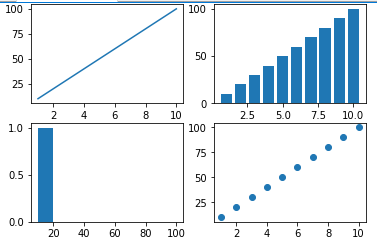
\includegraphics[width=5cm]{figures/6/1174073/teori/satu.png}
    \centering
    \caption{SubPlot}
\end{figure}

\item sebutkan semua pparameter color yang bisa digunakan contoh: m,c,r,k,...

Untuk parameter color yang bisa digunakan terdiri dari 2 type warna.

Tipe Warna RGB

Untuk keterangannya sebagai berikut
\begin{enumerate}
\item R untuk warna Red atau Merah
\item G untuk warna Green atau Hijau
\item B untuk warna Blue atau Biru
\end{enumerate}
Tipe warna CMYK

Untuk keterangannya sebagai berikut
\begin{enumerate}
\item    C untuk warna Cyan atau Biru Muda
\item    M untuk warna Mangenta atau Merah Tua
\item    Y untuk warna Yellow Atau Kuning
 \item   K untuk warna blacK atau Hitam
\end{enumerate}

\item Jelaskan bagaimana cara kerja dari fungsi hist, sertakan ilustrasi dan gambar sendiri?

Untuk fungsi histogram ini kedua titik koordinat boleh tidak sama. Misalnya x nya ada 10 nilai sedangkan Y nya ada 5 nilai, itu tidak akan jadi masalah karena diagram ini digunakan untuk mendata usia dari rentang tertentu atau kebutuhan lainnya.
Ini merupakan contoh dari penggunaan histogram
\lstinputlisting[firstline=27, lastline=34]{src/6/1174073/teori/1174073.py}
dan ini merupakan grafik histogram tersebut.
\begin{figure}[H]	
    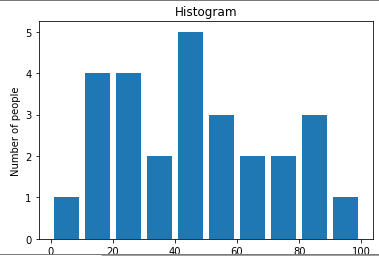
\includegraphics[width=5cm]{figures/6/1174073/teori/histogram.png}
    \centering
    \caption{Diagram Histogram}
\end{figure}

\item jelaskan lebih mendalam tentang parameter dari fungsi pie diantaranya labels, colors,startangle, shadow, explode, autopct.

Berikut penjelasan tentang parameter yang ada dalam pie chart
\begin{itemize}
    \item label
    Label digunakan untuk mempermudah pembaca dalam membaca diagram pie
    \item color
    warna digunakan untuk membedakan antar data
    \item startangle
    Digunakan untuk sudut yang digunakan untuk memulai diagram pie tersebut
    \item shadow
    bayangan digunakan untuk membuat bayangan dari setiap diagram pie yang menonjol
    \item explode
    explode digunakan untuk mengeluarkan suatu data agar data tersebut terlihat menonjol
    \item autopct
    Digunakan sesuai dengan berapa angka dibelakang koma yang kita inginkan
\end{itemize} 
\end{enumerate}